qsection{Experimental Results}
\label{sec:eval}
In this section, we first give some statistics of
our corpus and the extracted causality network, and evaluate the
quantity and quality of the cue patterns used in the extraction.
We then compared our results on the main COPA task against a number of
existing works using various other data sources and knowledge bases.
Next, we evaluate causality reasoning
on two additional tasks using the data from ConceptNet 4 to
further showcase the power of our framework.
Finally, we demonstrate our network's ability to identify causal directions
using annotated corpus of SemEval-2010 task 8, despite being
agnostic about the context of the input word pairs.
We release the evaluation data used in these experiments
at \url{http://202.120.38.146/causal}.

\subsection{Data Set and Extraction of Causality Network}
\label{sec:causalnet}
\begin{figure*}[th]
\centering
%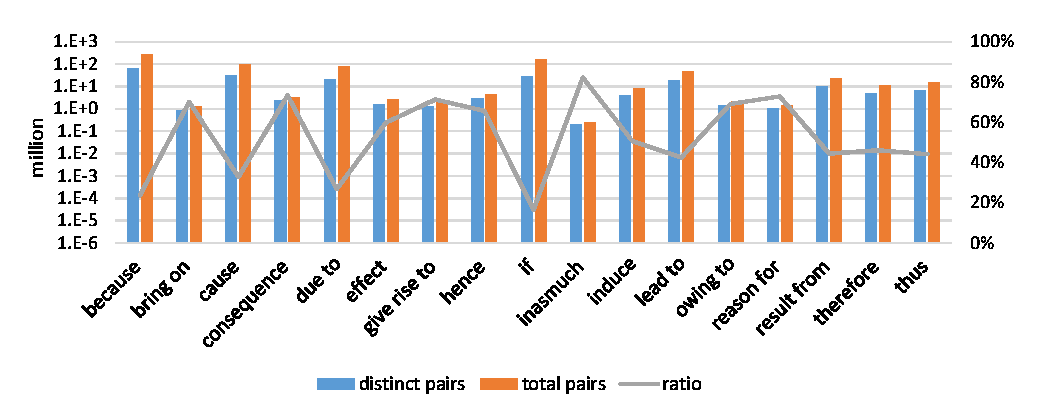
\epsfig{file=pattern1.eps, width=1.6\columnwidth}
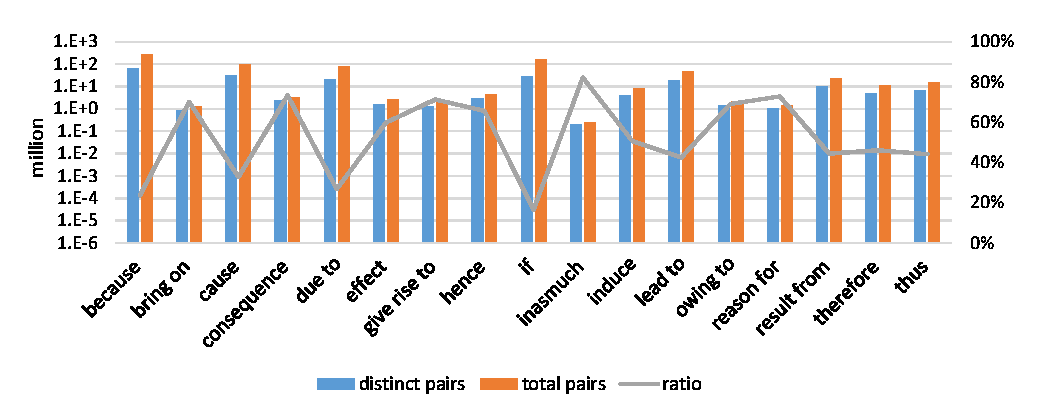
\includegraphics[width=1.6\columnwidth]{pattern1}
\caption{Number of (distinct) pairs extracted by cues}
\label{fig:pattern1}
\end{figure*}
We extracted our term causality network, which we call ``CausalNet''
for convenience in this section, from a large web text corpus (approximately
10TB), %The snapshot was generated in February, 2013
which contains about 1.6 billion web pages.
We extract 62,675,002 distinct causality evidences (e.g., causal pairs
or edges in CausalNet) from this corpus.
The average frequency of these evidences is 10.54.
The number of unique lemmatized terms (nodes)
in these evidences is 64,436, covering 41.49\% (64,436/155,287) of the
words in WordNet.

As a comparison, we separately extracted an
``event-based'' CausalNet using dependency relations~\cite{chen2014fast}
such as \emph{advmod} and \emph{dobj}.
Only bigram-phrases that match these relations and appear more than
20,000 times in the corpus are considered events; otherwise they are split
into words and paired up as before.
The average frequency on the edges of this event-based CausalNet
is 1.59, much smaller than the orginal CausalNet,
which would make our metric inaccurate due to its sparsity.
Therefore, subquent
experiments are done on the term-based CausalNet.

The 53 causal cues we used can be grouped into 17 sets, each
containing cues of the same meaning or lemma form but with different
tenses. Word pair distribution over these sets is shown in Figure
\ref{fig:pattern1}. The blue bars (left) are the number of distinct
pairs and the orange ones (right) show the total number of pairs.
Inter-sentence cues like ``if'' and ``because'' harvested the
largest number of pairs. But more specialized patterns such as
``reason'' and ``inasmuch'' find more diverse pairs, since the
number of distinct pairs is relatively large compared to the total
pairs extracted.
We show such diversity by the ratio between number of distinct pairs
and number of total pairs
and this ratio is marked by gray line in \figref{fig:pattern1}.

\begin{figure*}[th]
\centering
%\epsfig{file=pattern2.eps, width=1.6\columnwidth}
\includegraphics[width=1.6\columnwidth]{pattern2}
\caption{Number of causal vs. non-causal pairs from ConceptNet covered by cues}
\label{fig:pattern2}
\end{figure*}
To evaluate the quality of the causal cues, we make use of the
manually labeled causal events in
ConceptNet~\cite{liu2004commonsense} as ground truth. ConceptNet 4
contains 74,336 unlemmatized English words, forming
375,135 unique concepts, which are connected by 610,397 relation edges.
Only some of these relations encode causal knowledge,
such as ``Causes'', ``CausesDesire'' and ``HasPrerequisite''.
The total number of such causal relations is 52,778.
Each causal relation also associates with a vote from volunteers.
Those pairs associated with positive votes are annotated as causal pairs
(e.g. (listen to music$_c$, relax$_e$) ),
while associated with negative votes are annotated as false causal pairs
(e.g. (listen to music$_c$, soda can$_e$) ).

Since the pairs from ConceptNet contain
phrases and not just words, we consider a pair ($x$, $y$)
($x$ and $y$ are text spans) to be covered by a
causal cue, if at least one word $u$ from $x$ and another word $v$ from
$y$ are extracted as cause word and effect word by the cue
from the web corpus.
\figref{fig:pattern2} shows that in general, our cues can
effectively distinguish between positive and negative causal pairs,
with the exception of ``hence'' and ``consequence'', both of which
represent relatively coarse-grained entailment relation.
Particularly good cues to distinguish the positive and negative
pairs are ``due to'' and ``induce''.

\subsection{End-to-end Evaluation on COPA}
COPA task consists of 1000 causal reasoning questions, divided into
development question set and test question set of 500 each.
The incorrect alternative was purposely set semantically
close to the premise, which makes this task more difficult for
purely associative methods. In this experiment, our parameter $\lambda$
was trained on the development set.
All the reported results are on test set.

To show the usefulness of our causality metric, denoted as $CS$,
we compare the end-to-end results on COPA with the
best known PMI statistics on the web corpus.
To solve COPA question with PMI, we pair the terms from
premise and alternative and choose the alternative
with a higher PMI.

We trained our $CS_{\lambda}$ metric
on the development set of COPA
for different data sources (i.e. web corpus and CausalNet).
That means we compute $CS$ based on lexico co-occurrences from web corpus,
while computing $CS$ based on causality co-occurrences from CausalNet.
During the training period,
$CS_{\lambda=0.9}$ and $CS_{\lambda=1.0}$ achieve the same best results
using CausalNet while $CS_{\lambda=0.5}$
performs the best using the web corpus on the development set.
Then we show the performance of these trained $CS$ metrics on test split of COPA.
\tabref{tab:evaluation} shows that
$CS_{\lambda = 0.5}$ on web data
(64.8\%) outperforms PMI with any window sizes.
\tabref{tab:evaluation} also compares $CS_{\lambda=1.0}$ on CausalNet
with several other approaches.
PMI Gutenberg~\cite{roemmele2011choice} uses PMI statistic calculated
from Project Gutenberg (16GB of English-language text).
UTDHLT~\cite{goodwin2012utdhlt} is the
result of SemEval-2012 Task 7 systems. They proposes two
approaches. The first one uses PMI over bigrams from LDC Gigaword corpus
(8.4 million documents) as a
feature. The second one treats the task as a classification
problem and combine the features used in the first approach with
some additional features to train an SVM model.
The ConceptNet approach was our own baseline to illustrate the power of
human curated knowledge. Here we fuzzy match
the events or concepts from ConceptNet in COPA sentences, and then compute
the causal strength between two COPA sentences by the scores(e.g.votes)
associate with
causal relations in ConceptNet.
23 out of 500 questions
on COPA test split are matched by ConceptNet,
and 18 of them are correctly answered,
by computing the causality strength between two COPA sentences
from the votes associate with causal relations in ConceptNet.
We just randomly select an answer
for mismatched questions.
The last PMI method~\cite{gordon2011commonsense}, which was also the
state-of-the-art previously (65.4\%), uses a large corpus of
personal stories (37GB of text) with a window of 25.
All competing systems were assessed based
on their accuracy on the 500 questions in the COPA test
split~\cite{gordon2012copa}. Results show that our new metric
$CS_{\lambda=0.9}$$_{/}$$_{1.0}$,
when used together with the automatically harvested CausalNet
achieves significantly better accuracy on the COPA task.

\begin{table}[th]
\small
\centering
\caption{COPA results comparison}
\label{tab:evaluation}
\begin{tabular}{llccc}
\hline
Data Source & Methods & Accuracy(\%) \\
\hline
Web corpus & PMI (W=5) & 61.6\% \\
& PMI (W=10) & 61.0\% \\
& PMI (W=15) & 60.4\% \\
& PMI (W=25) & 61.2\% \\
& {\bf $CS_{\lambda=0.5}$} & {\bf 64.8\%} \\
\hline
Gutenberg & PMI (W=5)  & 58.8\% \\
& PMI (W=25) & 58.6\% \\
\hline
LDC Gigaword & UTDHLT Bigram PMI & 61.8\% \\
 & UTDHLT SVM & 63.4\% \\
\hline
ConceptNet & Fuzzy match & 51.3\% \\
\hline
1-Million Stories & PMI (W=25) & 65.2\% \\
10-Million Stories & PMI (W=25) & {\bf 65.4\%} \\ \hline
CausaNet & {\bf $CS_{\lambda = 1.0}$ } & {\bf 70.2} \%  \\
\hline
\end{tabular}
\end{table}

To further illustrate the effect of web data size on
commonsense causal reasoning, we randomly sample
20\%, 40\%, 60\% and 80\% of our web corpus and thus construct
various CausalNets of increasing sizes. The accuracies of
COPA evaluation using these knowledge bases with $CS_{\lambda=0.9}$
and $CS_{\lambda=1.0}$ are shown in \figref{fig:scale}.
One can observe a general positive correlation between the size of the data
and the ability to reason about commonsense causality. Even at 100\%,
that is the whole of the web corpus available to us, this trend shows
no signs of diminishing, which means, given more data, the results may be
even better. The curves in \figref{fig:scale} also shows a
small bump at 60\% of data.
This is probably due to the randomness in the data distribution (e.g., the
inclusion of certain type of web pages) and doesn't change the overall
scalability of our framework.

\begin{figure}[htb]
\centering
%\epsfig{file=pic2.eps, width=0.9\columnwidth}
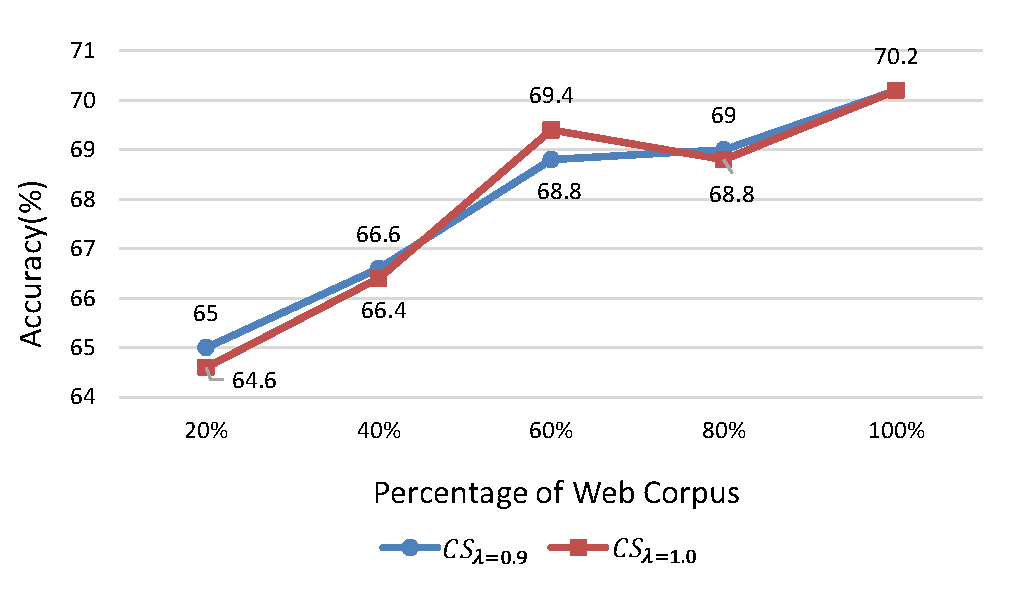
\includegraphics[width=0.9\columnwidth]{causalnet_scales}
\caption{COPA evaluation on different scales of CausalNet}
\label{fig:scale}
\end{figure}

To understand the effect of $\lambda$ in our metric on
causal reasoning, we conduct more experiments on COPA using different values
of $\lambda$, and on both web corpus and CausalNet. As baselines,
we also include the results using conditional probabilities in
dual directions, $p(i_c | j_e)$ and $p(j_e | i_c)$. The results
are shown in \tabref{tab:varcs}.
Generally, conditional probability underperforms in this task for
both data sources. When computing causal strength using implicit
causality evidences,
the web data is largely unbiased and hence
the causality evidences are observed with roughly
equal sufficiency and necessity causality. Therefore $\lambda=0.5$ gives the best result.
\ZY{In contrast, when computing $CS$ from CausalNet which is biased
by the explicit causality patterns.}
People rarely state ``\textit{A causes B}'' in text explicitly,
when \textit{A} apparently implies \textit{B}.
Therefore, sufficiency causality is seldom
observed, hence a larger $\lambda$ value gives better results.

\begin{table}[th]
\small
\centering
\caption{COPA results for different CS variants}
\label{tab:varcs}
\begin{tabular}{llc}
\hline
Data Source & Methods & Accuracy(\%) \\
\hline
Web corpus & $p(j_e | i_c)$ & 58.2\%\\
 & $p(i_c | j_e)$ & 62.8\% \\
 & $CS_{\lambda=0.5}$ & {\bf 64.8\%} \\
 & $CS_{\lambda=0.7}$ & 63.4\% \\
 & $CS_{\lambda=0.9}$ & 63.0\% \\
 & $CS_{\lambda=1.0}$ & 63.0\% \\
 \hline
CausalNet & $p(j_e | i_c)$ & 56.2\% \\
 & $p(i_c | j_e)$ & 60.2\% \\
 & $CS_{\lambda=0.5}$ & 68.8\% \\
 & $CS_{\lambda=0.7}$ & 69.4\% \\
 & $CS_{\lambda=0.9}$ & {\bf 70.2\%} \\
 & $CS_{\lambda=1.0} $ & {\bf 70.2\%} \\
\hline
\end{tabular}
\end{table}

\subsection{Causality Detection}

Causality detection, or identifying the causal relation in text is
an important task for many applications, such as event prediction,
risk analysis, or decision making support\cite{mirza2014extracting}.
To show the effectiveness of our work in this aspect,
we investigate the following two research questions on
CausalNet, using data from ConceptNet4.
\begin{itemize}
\item {\bf RQ1:}
For arbitrary event pair manually labeled as \emph{causal} (positive data)
or \emph{non-causal} (negative data), we investigate whether our
proposed causality strength score clearly separates the two.
\item {\bf RQ2:} Inspired by COPA, we select causal and non-causal pairs
sharing the same premise from ConceptNet and form two-choice
questions, to evaluate the ability of CausalNet in selecting the
correct choice.
\end{itemize}

For {\bf RQ1,}
we use the same 200 causal and non-causal event pairs from
\figref{fig:pattern2} as positive and negative data.
\figref{fig:conceptApp1}
%\figref{fig:rq1-0.9} and \figref{fig:rq1-1.0}
shows the causality score $CS_{\lambda=0.9}$ and $CS_{\lambda=1.0}$ ($y$-axis)
of 100 positive
and negative pairs indexed randomly ($x$-axis).
We can observe that scores
of positive and negative pairs are accurately distinguished by a
linear function, %$y=10^{0}$
$y=0.7$, indicated by the gray line.
Consequently, existing systems for causality identification and detection
can incorporate our work to improve their accuracy.

\begin{figure*}[ht!]
\centering
\begin{subfigure}[t]{0.9\columnwidth}
\centering
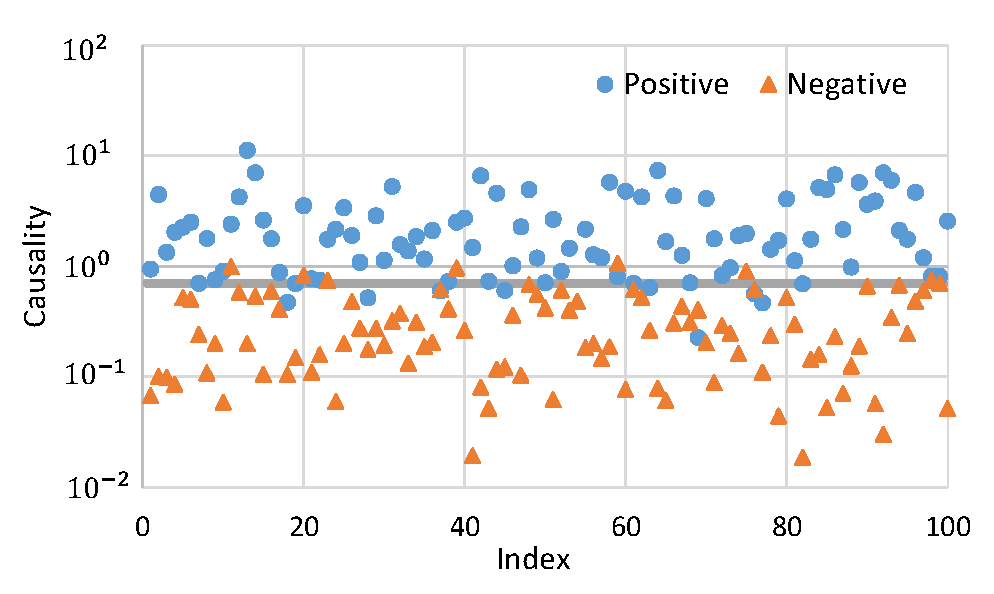
\includegraphics[width=0.9\columnwidth]{rq1-a}
\caption{$CS_{\lambda=0.9}$}
\end{subfigure}
\begin{subfigure}[t]{0.9\columnwidth}
\centering
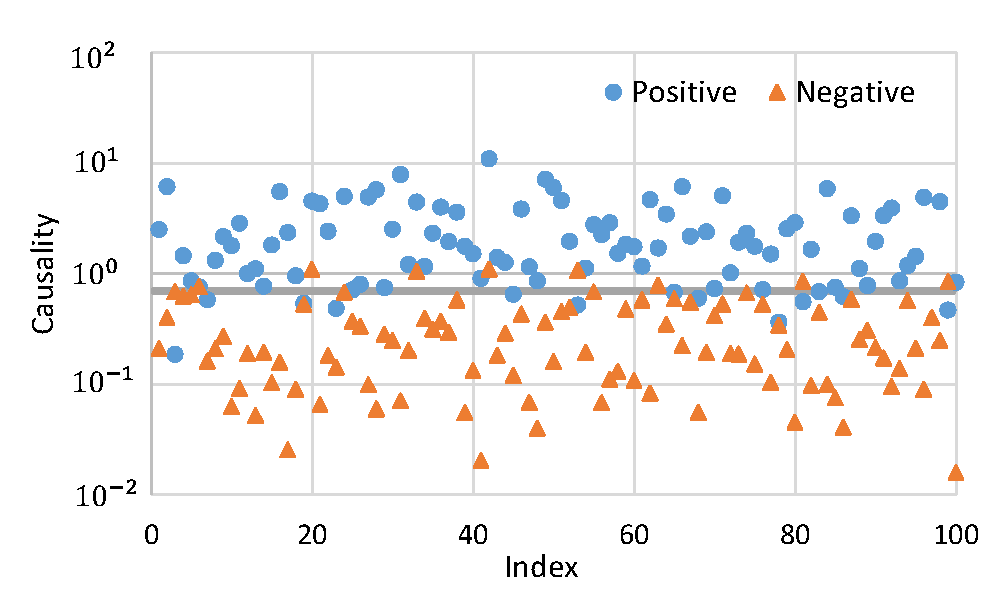
\includegraphics[width=0.9\columnwidth]{rq1-b}
\caption{$CS_{\lambda=1.0}$}
\end{subfigure}
\caption{Distinguishing causality on ConceptNet}
\label{fig:conceptApp1}
\end{figure*}

For {\bf RQ2,}
due to sparsity of pairs sharing the same premise,
we follow \emph{pseudo-disambiguation task} in~\cite{Erk}.
In particular, we use \emph{Causes} relationship $(i,j)$ with
positive votes, such that $i$ is the shared premise and $j$ is a
positive alternative. We then generate a negative alternative by
randomly selecting $j'$ without \emph{Causes} relationship with $i$.
Since ConceptNet does not exhaustively
label all possible causal relationships, randomly selected $j'$ can
be actually causal, i.e., \emph{false negatives} may exist. In such
situation, we removed the question involving such false negative,
and consequently obtained a dataset of 412 questions in which 259
look for an effect while 153 look for a cause. \tabref{tab:rq2}
shows that the results of different $CS_\lambda$
using CausalNet.

\begin{table}[th]
%\small
\centering
\caption{Result of ConceptNet RQ2}
\begin{tabular}{cc}
\hline
Methods & Accuracy(\%) \\
\hline
$CS_{\lambda=0.5}$ & 78.4\%  \\
$CS_{\lambda=0.9}$ & 78.6\%  \\
$CS_{\lambda=1.0}$ & 78.6\%  \\
\hline
\end{tabular}
\label{tab:rq2}
\end{table}

\subsection{Direction of Causality}
\begin{table*}[bht]
\centering
\caption{Random samples of annotated causal pairs from SemEval-2010 task 8}
\label{tab:sample}
%\footnotesize
\small
\begin{tabular}{| l c | l c |}
\hline \multicolumn{2}{|c|}{Pairs with match in CausalNet} &
\multicolumn{2}{c|}{Pairs without match in CausalNet}\\
\hline
\multicolumn{1}{|c}{Causal Pair} & \multicolumn{1}{c|}{Commonsense} & \multicolumn{1}{|c}{Causal Pair} & \multicolumn{1}{c|}{Commonsense} \\
\hline
$(\text{vaccine}_c, \text{fever}_e)$ & Yes & $(\text{drink}_c, \text{suffering}_e)$ & Yes\\
$(\text{tension}_c, \text{headache}_e)$ & Yes  & $(\text{malfunction}_c, \text{inflammation}_e)$ & No \\
$(\text{passage}_c, \text{noise}_e)$ & Yes & $(\text{growth}_c, \text{inflammation}_e)$ & No\\
$(\text{injury}_c, \text{discomfort}_e)$ & Yes & $(\text{pie}_c, \text{poison}_e)$ & No \\
$(\text{ash}_c, \text{drama}_e)$ & No & $(\text{city}_c, \text{anger}_e)$ & No \\
$(\text{extraction}_c, \text{extinction}_e)$ & Yes & $(\text{infection}_c, \text{acne}_e)$ & Yes \\
$(\text{mess}_c, \text{crisis}_e)$ & Yes & $(\text{institution}_c, \text{fraud}_e)$ & No \\
$(\text{pinworm}_c, \text{infestation}_e)$ & Yes & $(\text{dog}_c, \text{joy}_e)$ & No \\
$(\text{parasite}_c, \text{toxoplasmosis}_e)$ & Yes & $(\text{fear}_c, \text{attack}_e)$ & No \\
$(\text{disability}_c, \text{benefit}_e)$ & Yes & $(\text{bacteria}_c, \text{acne}_e)$ & Yes \\
$(\text{elimination}_c, \text{riot}_e)$ & Yes & $(\text{fireplace}_c, \text{warmth}_e)$ & Yes \\
$(\text{generator}_c, \text{signal}_e)$ & Yes & $(\text{tax}_c, \text{fluctuation}_e)$ & No \\
$(\text{drug}_c, \text{unconsciousness}_e)$ & Yes & $(\text{bacteria}_c, \text{breakout}_e)$ & Yes \\
$(\text{zinc}_c, \text{growth}_e)$ & Yes & $(\text{injury}_c, \text{operation}_e)$ & Yes \\
$(\text{reaction}_c, \text{inversion}_e)$ & Yes & $(\text{pregnancy}_c, \text{nausea}_e)$ & Yes \\
$(\text{movement}_c, \text{earthquake}_e)$ & Yes & $(\text{attack}_c, \text{shock}_e)$ & Yes \\
$(\text{virus}_c, \text{disease}_e)$ & Yes & $(\text{lack}_c, \text{reliance}_e)$ & No \\
$(\text{drum}_c, \text{sound}_e)$ & Yes & $(\text{computer}_c, \text{radiation}_e)$ & No \\
$(\text{vaccine}_c, \text{outbreak}_e)$ & Yes & $(\text{ointment}_c, \text{discomfort}_e)$ & No \\
$(\text{press}_c, \text{reaction}_e)$ & Yes & $(\text{ginseng}_c, \text{taste}_e)$ & No \\

\hline
\end{tabular}
\end{table*}

Given a pair of terms $i$ and $j$ that are causally related,
CausalNet can generally tell whether the causality is encoded by $(i_c,j_e)$
or by $(j_c,i_e)$ in common sense, without the context of
$i$ and $j$. In other words, as we will show next, CausalNet
provides a reasonable prior knowledge of causality direction.
We use the annotated corpus of SemEval-2010 Task 8 to evaluate this.
There are 920 pairs of terms annotated as Cause-Effect relationship in
SemEval-2010 Task 8 training corpus. CausalNet covered 894 out of
920 pairs (97.2\%).
Each Cause-Effect pair in the SemEval data set is annotated as follows:
\begin{itemize}
  \item[] Sentence:\\
  {\em I too, get a $\langle e1\rangle$ \textbf{headache}$\langle/e1\rangle$
  from $\langle e2\rangle$ \textbf{wine}$\langle/e2\rangle$, and was always told that it was the sulfites.}
  \item[] Relation: \\ \emph{Cause-Effect($e2$,$e1$)}
\end{itemize}
In the above example, $e1$ represents the term ``headache'', and
$e2$ represents ``wine''. The relation Cause-Effect($e2$,$e1$)
indicates that the causality encoded in this sentence is
$(\text{wine}_c,\text{headache}_e)$,
but not
$(\text{headache}_c,\text{wine}_e)$.
We can obtain this useful
insight by the prior knowledge from CausalNet.
We simply compare the causal strength of
$(i_c,j_e)$ with that of $(j_c,i_e)$ provided by
CausalNet. If $CS(i_c,j_e) > CS(j_c,i_e)$, we
conclude that the causality is encoded by $(i_c,j_e)$,
otherwise the causality is encoded by $(j_c,i_e)$.

The agreement between CausalNet and annotated ground truth in SemEval-2010
Task 8 is 82.3\%, i.e., 736 out of 894 pairs from SemEval find
a matching pair in the same causal direction from CausalNet.
\tabref{tab:sample} shows 20 random samples of annotated causal pairs
from SemEval-2010 Task 8 corpus. 10 of those are matched by
CausalNet and the rest are not. Three human judges were employed to
mark whether these pairs follow common sense or not. \ZY{The pairs
are considered common sense by at least 2 judges.}
We can see that all but one pairs in the left column are common sense,
while most of those pairs in the right column are not common sense.
This means, where CausalNet predicts correctly, it is really due to the power
of commonsense knowledge. On the other hand, CausalNet makes mistakes primarily
due to the lack of context in small amount of cases, and not because the
knowledge enclosed is wrong.
